%% LyX 2.3.4.2 created this file.  For more info, see http://www.lyx.org/.
%% Do not edit unless you really know what you are doing.
\documentclass[english,dvipsnames,aspectratio=169]{beamer}
\usepackage{mathptmx}
\usepackage{eulervm}
\usepackage[T1]{fontenc}
\usepackage[latin9]{inputenc}
\usepackage{babel}
\usepackage{amstext}
\usepackage{amssymb}
\usepackage{graphicx}
\usepackage{ifthen}
\usepackage{xcolor}
\usepackage{xspace}
\usepackage{tikz}
\usetikzlibrary{tikzmark}
\usetikzlibrary{calc}
\usepackage{pgfplots}
%\pgfplotsset{compat=1.17}
\usepackage{booktabs}
\usepackage{xpatch}

\usepackage{pgfpages}
\setbeamertemplate{note page}{\pagecolor{yellow!5}\insertnote}
%\setbeameroption{hide notes} % Only slides
%\setbeameroption{show only notes} % Only notes
%\setbeameroption{show notes on second screen=right} % Both


\xpatchcmd{\itemize}
  {\def\makelabel}
  {\ifnum\@itemdepth=1\relax
     \setlength\itemsep{2ex}% separation for first level
   \else
     \ifnum\@itemdepth=2\relax
       \setlength\itemsep{1ex}% separation for second level
     \else
       \ifnum\@itemdepth=3\relax
         \setlength\itemsep{0.5ex}% separation for third level
   \fi\fi\fi\def\makelabel
  }
 {}
 {}

\ifx\hypersetup\undefined
  \AtBeginDocument{%
    \hypersetup{unicode=true,pdfusetitle,
 bookmarks=true,bookmarksnumbered=false,bookmarksopen=false,
 breaklinks=false,pdfborder={0 0 0},pdfborderstyle={},backref=false,colorlinks=true,
 allcolors=NYUPurple,urlcolor=LightPurple}
  }
\else
  \hypersetup{unicode=true,pdfusetitle,
 bookmarks=true,bookmarksnumbered=false,bookmarksopen=false,
 breaklinks=false,pdfborder={0 0 0},pdfborderstyle={},backref=false,colorlinks=true,
 allcolors=NYUPurple,urlcolor=LightPurple}
\fi

\makeatletter

%%%%%%%%%%%%%%%%%%%%%%%%%%%%%% LyX specific LaTeX commands.
%% Because html converters don't know tabularnewline
\providecommand{\tabularnewline}{\\}

%%%%%%%%%%%%%%%%%%%%%%%%%%%%%% Textclass specific LaTeX commands.
% this default might be overridden by plain title style
\newcommand\makebeamertitle{\frame{\maketitle}}%
% (ERT) argument for the TOC
\AtBeginDocument{%
  \let\origtableofcontents=\tableofcontents
  \def\tableofcontents{\@ifnextchar[{\origtableofcontents}{\gobbletableofcontents}}
  \def\gobbletableofcontents#1{\origtableofcontents}
}

%%%%%%%%%%%%%%%%%%%%%%%%%%%%%% User specified LaTeX commands.
\usetheme{CambridgeUS} 
\beamertemplatenavigationsymbolsempty


% Set Color ==============================
\definecolor{NYUPurple}{RGB}{87,6,140}
\definecolor{LightPurple}{RGB}{165,11,255}


\setbeamercolor{title}{fg=NYUPurple}
\setbeamercolor{frametitle}{fg=NYUPurple}

\setbeamercolor{background canvas}{fg=NYUPurple, bg=white}
\setbeamercolor{background}{fg=black, bg=NYUPurple}

\setbeamercolor{palette primary}{fg=black, bg=gray!30!white}
\setbeamercolor{palette secondary}{fg=black, bg=gray!20!white}
\setbeamercolor{palette tertiary}{fg=gray!20!white, bg=NYUPurple}

\setbeamertemplate{headline}{}
\setbeamerfont{itemize/enumerate body}{}
\setbeamerfont{itemize/enumerate subbody}{size=\normalsize}

\setbeamercolor{parttitle}{fg=NYUPurple}
\setbeamercolor{sectiontitle}{fg=NYUPurple}
\setbeamercolor{sectionname}{fg=NYUPurple}
\setbeamercolor{section page}{fg=NYUPurple}
%\setbeamercolor{description item}{fg=NYUPurple}
%\setbeamercolor{block title}{fg=NYUPurple}

\setbeamertemplate{blocks}[rounded][shadow=false]
\setbeamercolor{block body}{bg=normal text.bg!90!NYUPurple}
\setbeamercolor{block title}{bg=NYUPurple!30, fg=NYUPurple}



\AtBeginSection[]{
  \begin{frame}
  \vfill
  \centering
\setbeamercolor{section title}{fg=NYUPurple}
 \begin{beamercolorbox}[sep=8pt,center,shadow=true,rounded=true]{title}
    \usebeamerfont{title}\usebeamercolor[fg]{title}\insertsectionhead\par%
  \end{beamercolorbox}
  \vfill
  \end{frame}
}

\makeatother

\setlength{\parskip}{\medskipamount} 

\input ../macros

\begin{document}
\input ../rosenberg-macros

\title[DS-GA 1003]{Discussion on Regularization}
\author{He He\\\vspace{2em}{
    Slides based on Lecture
    \href{https://davidrosenberg.github.io/mlcourse/Archive/2019/Lectures/03a.elastic-net.pdf}{3a}
    from David Rosenberg's \href{https://github.com/davidrosenberg/mlcourse}{course material}.
}}

\date{Feb 16, 2021}
\institute{CDS, NYU}

\makebeamertitle
\mode<article>{Just in article version}

\begin{frame}
    {Logistics}
    \begin{itemize}
        \item Thanks for the course feedback!
        \item Piazza posting instructions
            \begin{itemize}
                \item Search for similar questions
                \item Describe your progress and clarify confusion points
            \end{itemize}
        \item Feel free to turn on video (when talking)
        \item Tutorial for convex optimization (preparation for SVM) 
            on \textbf{Thursday 9:30am--10:30am} during Marylou's OH
            \begin{itemize}
                \item Convex functions
                \item Primal/Dual problem, strong/weak duality
                \item Complementary slackness, KKT conditions
            \end{itemize}
    \end{itemize}
\end{frame}

\section{Model Selection}

\begin{frame}
    {Feature Selection}
    \begin{itemize}
        \item \head{Goal}: Select the ``best'' subset of features according to some \textbf{score}
            \begin{itemize}
                \item Can also be formulated as $\ell_0$ regularization
                \item $\ell_0$ ``norm'': number of non-zero elements
                \item \textbf{Forward/Backward selection} is a greedy method often used in practice
            \end{itemize}
        \item Pitfalls in feature selection
            \begin{itemize}
                \item Is it possible to include irrelevant features (false positives)?
                    \note[item]{Yes, especially if we use validation error as the score, because an irrelevant feature that has a tiny effect can improve validation error by chance. It's less likely to happen with $\ell_0$ penalty, because each addition feature must improve the loss by at least $\lambda$.}
                \item What happens when we have dependence among features (e.g. colinearity)?
                    \note[item]{It will take either or both. The selected features may not be causal. For example, a confounding variable makes irrelevant features look relevant. In general, the effectiveness of a feature must be interpreted in the context of other features.}
            \end{itemize}
    \end{itemize}
\end{frame}

\begin{frame}
    {Model Selection}
    \begin{itemize}
        \item Feature selection is a special case of \textbf{model selection}:
            \begin{itemize}
                \item Degree of the polynomial function
                \item Decision tree vs kNN
                \item More broadly, hyperparameters of learning algorithms
            \end{itemize}
        \item We need to assess the performance of the model in order to select the ``best'' one
            \begin{itemize}
                \item Can we use the training error?
                    \note[item]{No, the training error always decreases if we increase the complexity of the hypothesis space.}
                \item What is the ideal performance measure?
            \end{itemize}
    \end{itemize}
\end{frame}

\begin{frame}
    {Test error}
    \begin{itemize}
        \item \textbf{Test error} (or \textbf{generalization error}) of a predictor $\hat{f}$:
            $$
            \BE_{P_{\sX\times\sY}}\pb{\ell(\hat{f}(x),y)} .
            $$
        \item Note that this is just the risk of $\hat{f}$.
        \item What we really care about is the test error, not the error on the test set!
        \item But we can use the test set error to estimate the test error.
        \item \al{Important}: the test set cannot influence training in \textit{any} way.
            \begin{itemize}
                \item Is it okay to look at the test set as long as the label is hidden?
                    \note[item]{No! Now that you've seen the test data, it will influence your model development, and we risk overfitting to the test set. You should only run on the test set at the end.}
            \end{itemize}
        \item For model selection, our goal is to estimate the test error of each model 
    \end{itemize}
\end{frame}

\begin{frame}
    {Estimate Test Error for Model Selection}
    In order to do model selection,\\
    \begin{itemize}
        \item We need to \hl{estimate test error}, but we cannot use the true test set.
        \item Best approach is to use a \textbf{validation set} (if we have enough data).
    \end{itemize}
    \medskip
    Other methods to estimate test error:\\
    \begin{itemize}
        \item Re-use training samples: create multiple train/test sets
            \begin{itemize}
                \item Cross validation, bootstrap
            \end{itemize}
        \item Training error + penalty 
            \begin{itemize}
                \item AIC, BIC, MDL
            \end{itemize}
    \end{itemize}
\end{frame}

\begin{frame}
    {Bias-Variance Decomposition}
    \begin{itemize}
        \item Note that the test error is a random variable. Why?
        \item Assume the true model is $y = f(x) + \epsilon$ and 
            $\BE{\epsilon} = 0$ and $\var(\epsilon)=\sigma^2$
        \item Consider the expected square loss over \textit{training sets}:
            \begin{align}
                \text{err}(x) &= 
                \BE\pb{\p{y - \hat{f}(x)}^2} \\
                &= \sigma^2 + \BE\pb{\hat{f}(x) - \BE\hat{f}(x)}^2
                + \pb{f(x) - \BE\hat{f}(x)}^2
            \end{align}
            \note[item]{irreducible error + variance($\hat{f}(x)$)
            + ($\text{bias}^2(\hat{f}(x))$)}
        \item Both excess risk decomposition and bias-variance decomposition analyze different sources of the test error
            and they lead to similar conclusions.
            \note[item]{Note that in this case, the irreducible error is the risk of the Bayes predictor.}
        \item What's the relation between complexity and bias/variance? 
    \end{itemize}
\end{frame}

\begin{frame}
    {Bias-Variance Trade-off}
    Training set error (blue) and test set error (red)
    \begin{figure}
        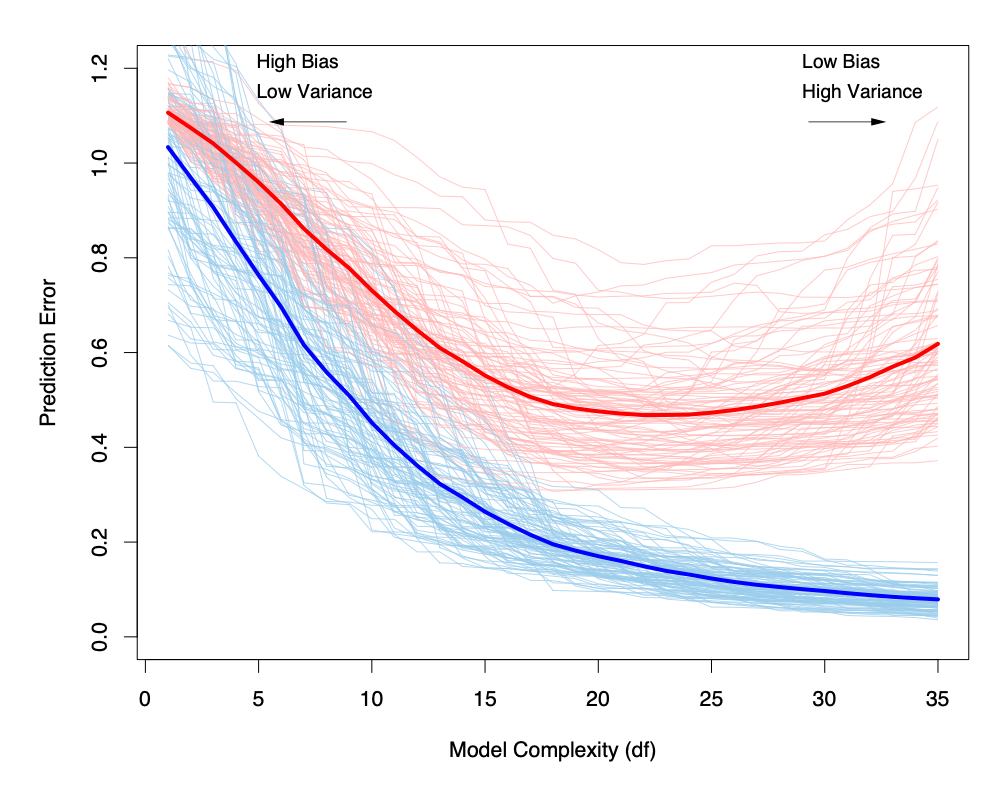
\includegraphics[height=0.7\textheight]{figures/bias-variance}
    \end{figure}
\end{frame}

\section{Regularization and Dependent Features}
\begin{frame}
    {$\ell_p$ Regularization}
        $\ell_0$ regularization (subset selection)
            $$
            f(w) = \|Xw - y\|^2 + \lambda \|w\|_0
            $$
        $\ell_1$ regularization (Lasso)
            $$
            f(w) = \|Xw - y\|^2 + \lambda \|w\|_1
            $$
        $\ell_2$ regularization (Ridge)
            $$
            f(w) = \|Xw - y\|^2 + \lambda \|w\|^2
            $$
    \begin{itemize}
        \item Which one(s) can be used for feature selection?
            \note[item]{L1 and L0. L1 is not as sparse as L0 though.}
        \item Which one(s) is fast to solve?
            \note[item]{L1 and L2. Descent-based methods.}
        \item Which one(s) gives unique solution?
            \note[item]{L2. L0 and L1 don't have unique solution given dependent features.}
    \end{itemize}
\end{frame}

\begin{frame}{Repeated features}
\begin{itemize}
\item Suppose we have one feature $x_{1}\in\reals$
and response variable $y\in\reals$.

\item Got some data and ran least squares linear regression.
The ERM is
\[
\hat{f}(x_{1})=4x_{1}.
\]

\item What is the ERM solution if we get a new feature $x_{2}$, 
but we always have $x_{2}=x_{1}$?
        \note[item]{$\hat{f}(x_{1},x_{2})=w_{1}x_{1}+w_{2}x_{2}$ is an ERM iff $w_{1}+w_{2}=4$}
        \vspace{5em}
\end{itemize}
\end{frame}

\begin{frame}{Duplicate Features: $\ell_{1}$ and $\ell_{2}$ norms}
\begin{itemize}
\item $\hat{f}(x_{1},x_{2})=w_{1}x_{1}+w_{2}x_{2}$ is an ERM iff $w_{1}+w_{2}=4$.

\item What if we introduce the $\ell_{1}$ and $\ell_{2}$ regularization:
\end{itemize}
\begin{center}
\begin{tabular}{|c|c|c|c|}
\hline 
$w_{1}$ & $w_{2}$ & $\|w\|_{1}$ & $\|w\|_{2}^{2}$\tabularnewline
\hline 
\hline 
4 & 0 & \hl{4} & 16\tabularnewline
\hline 
2 & 2 & \hl{4} & \hl{8}\tabularnewline
\hline 
1 & 3 & \hl{4} & 10\tabularnewline
\hline 
-1 & 5 & 6 & 26\tabularnewline
\hline 
\end{tabular}
\end{center}

\begin{itemize}
\item $\|w\|_{1}$ doesn't discriminate, as long as all have same sign
\item $\|w\|_{2}^{2}$ minimized when weight is spread equally
\item Picture proof: What does the level sets of ERM look like?
\end{itemize}
\end{frame}

\begin{frame}{Equal Features, $\ell_{2}$ Constraint}
\begin{center}
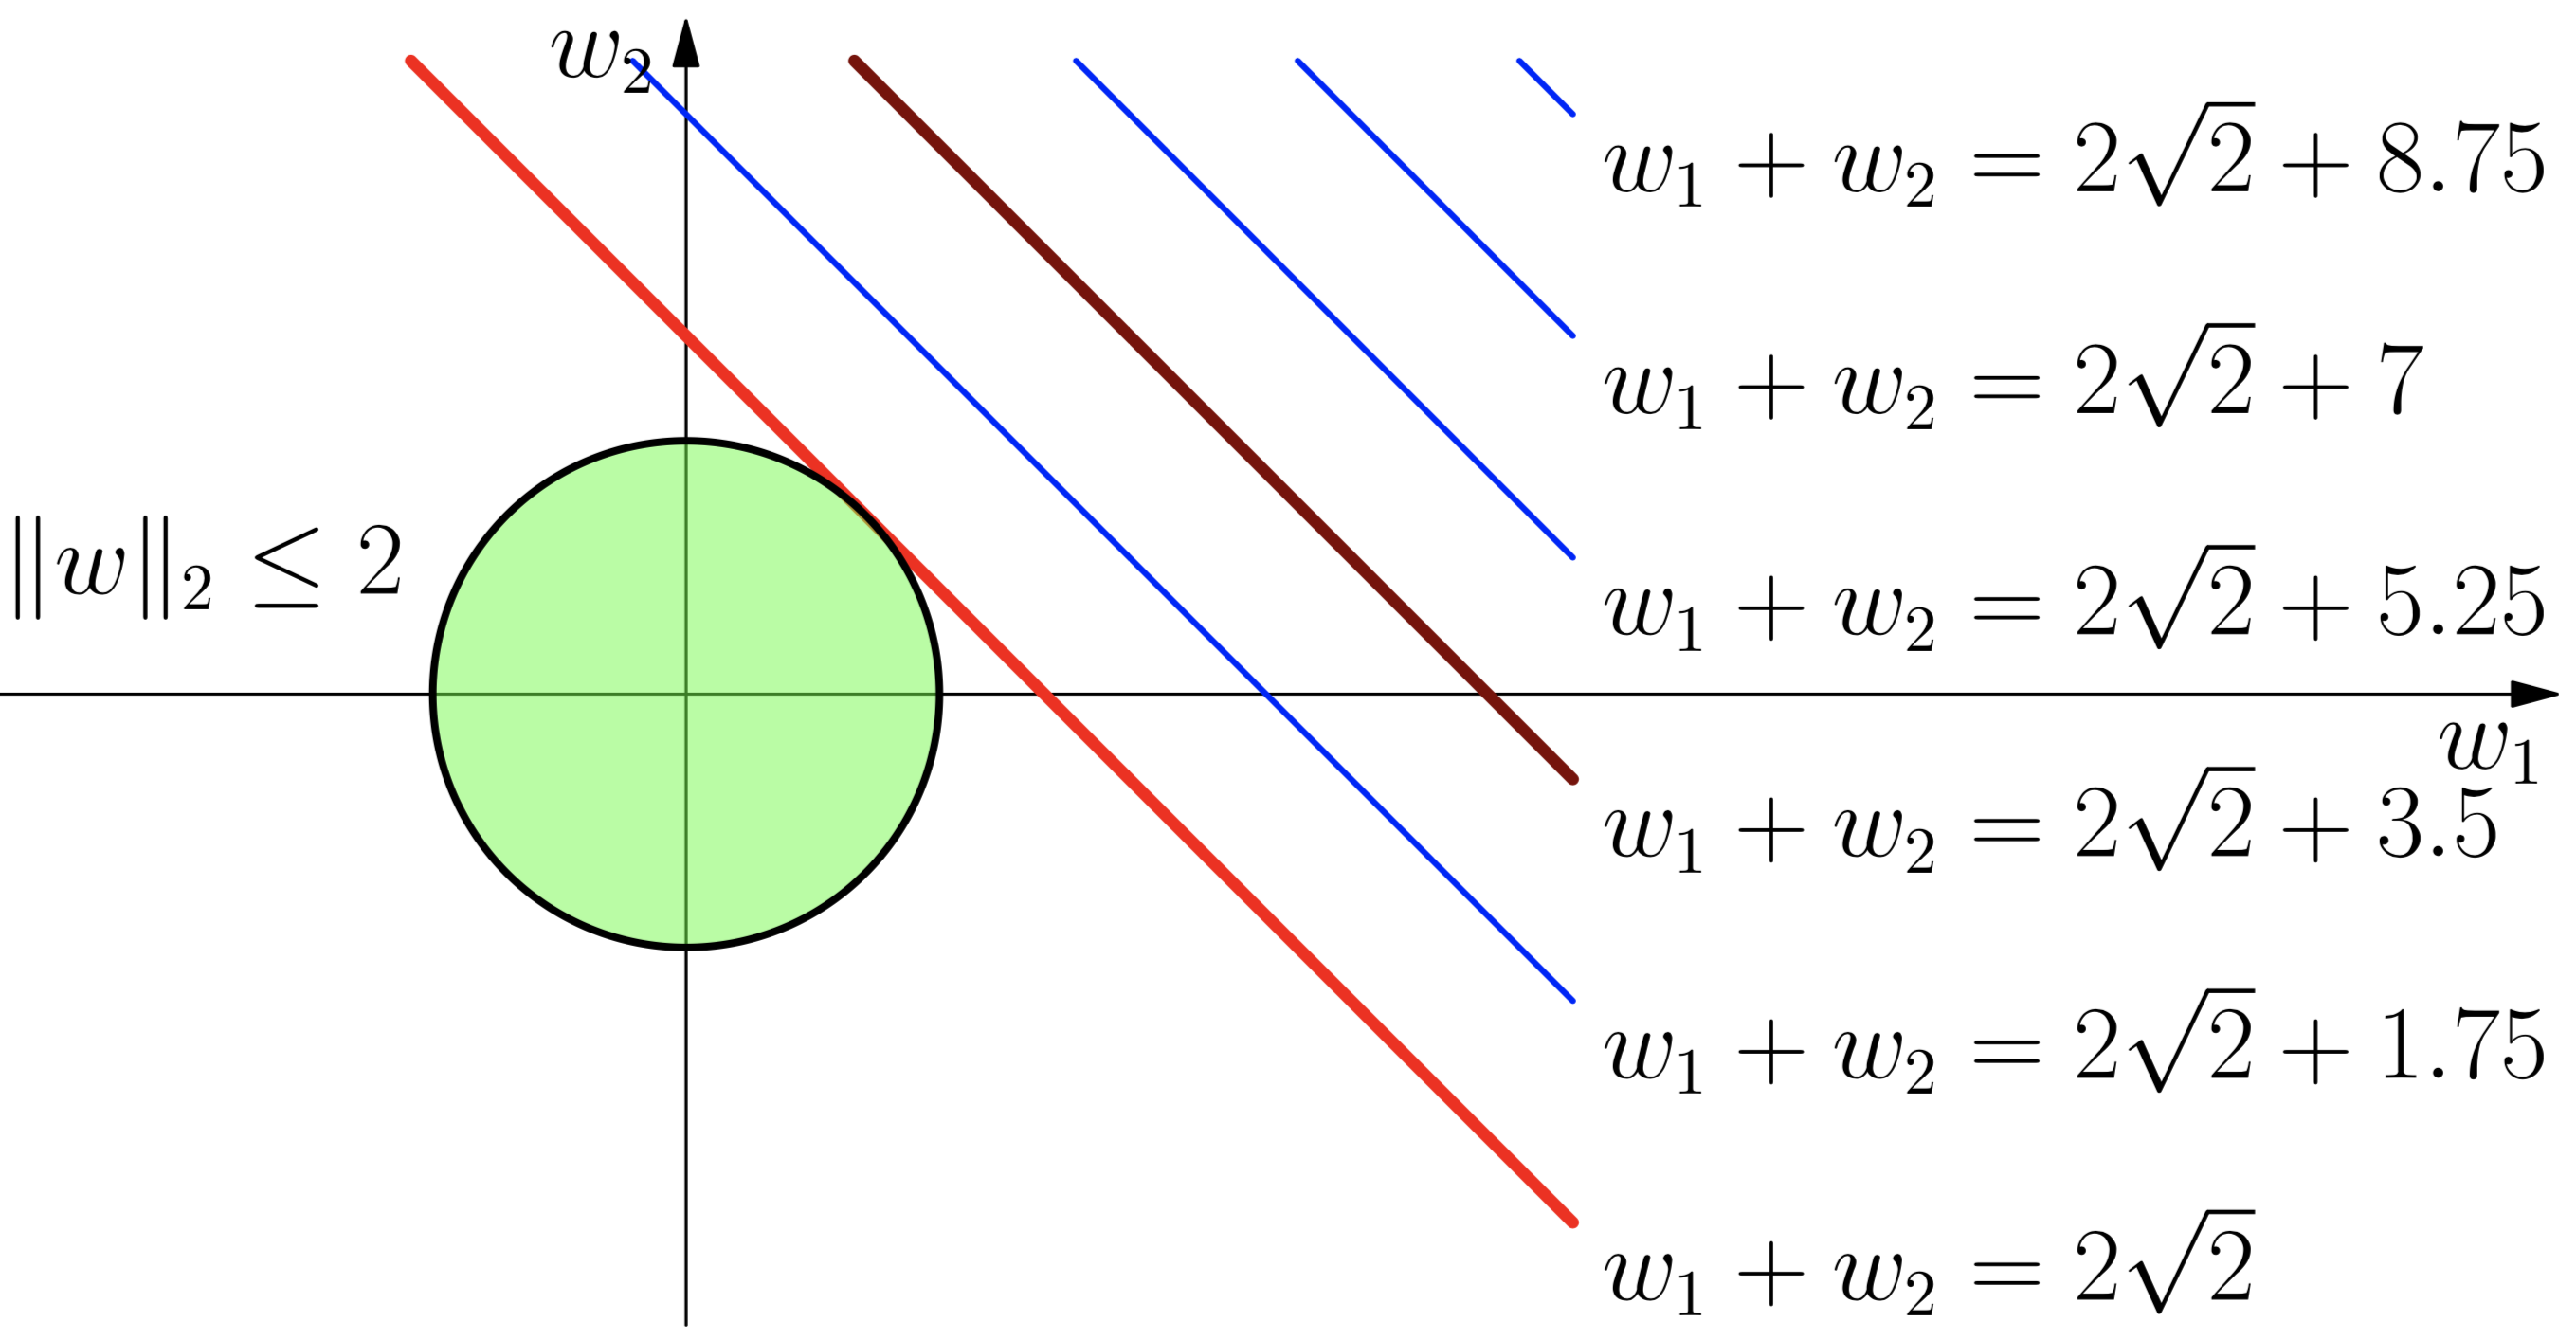
\includegraphics[height=0.4\textheight]{figures/L2Eq}
\par\end{center}
\begin{itemize}
\item Suppose the line $w_{1}+w_{2}=2\sqrt{2}+3.5$ corresponds to the empirical
risk minimizers.
\item Empirical risk increase as we move away from these parameter settings
\item Intersection of $w_{1}+w_{2}=2\sqrt{2}$ and the norm ball $\|w\|_{2}\le2$
is ridge solution.
\item Note that $w_{1}=w_{2}$ at the solution
\end{itemize}
\end{frame}
%
\begin{frame}{Equal Features, $\ell_{1}$ Constraint}
\begin{center}
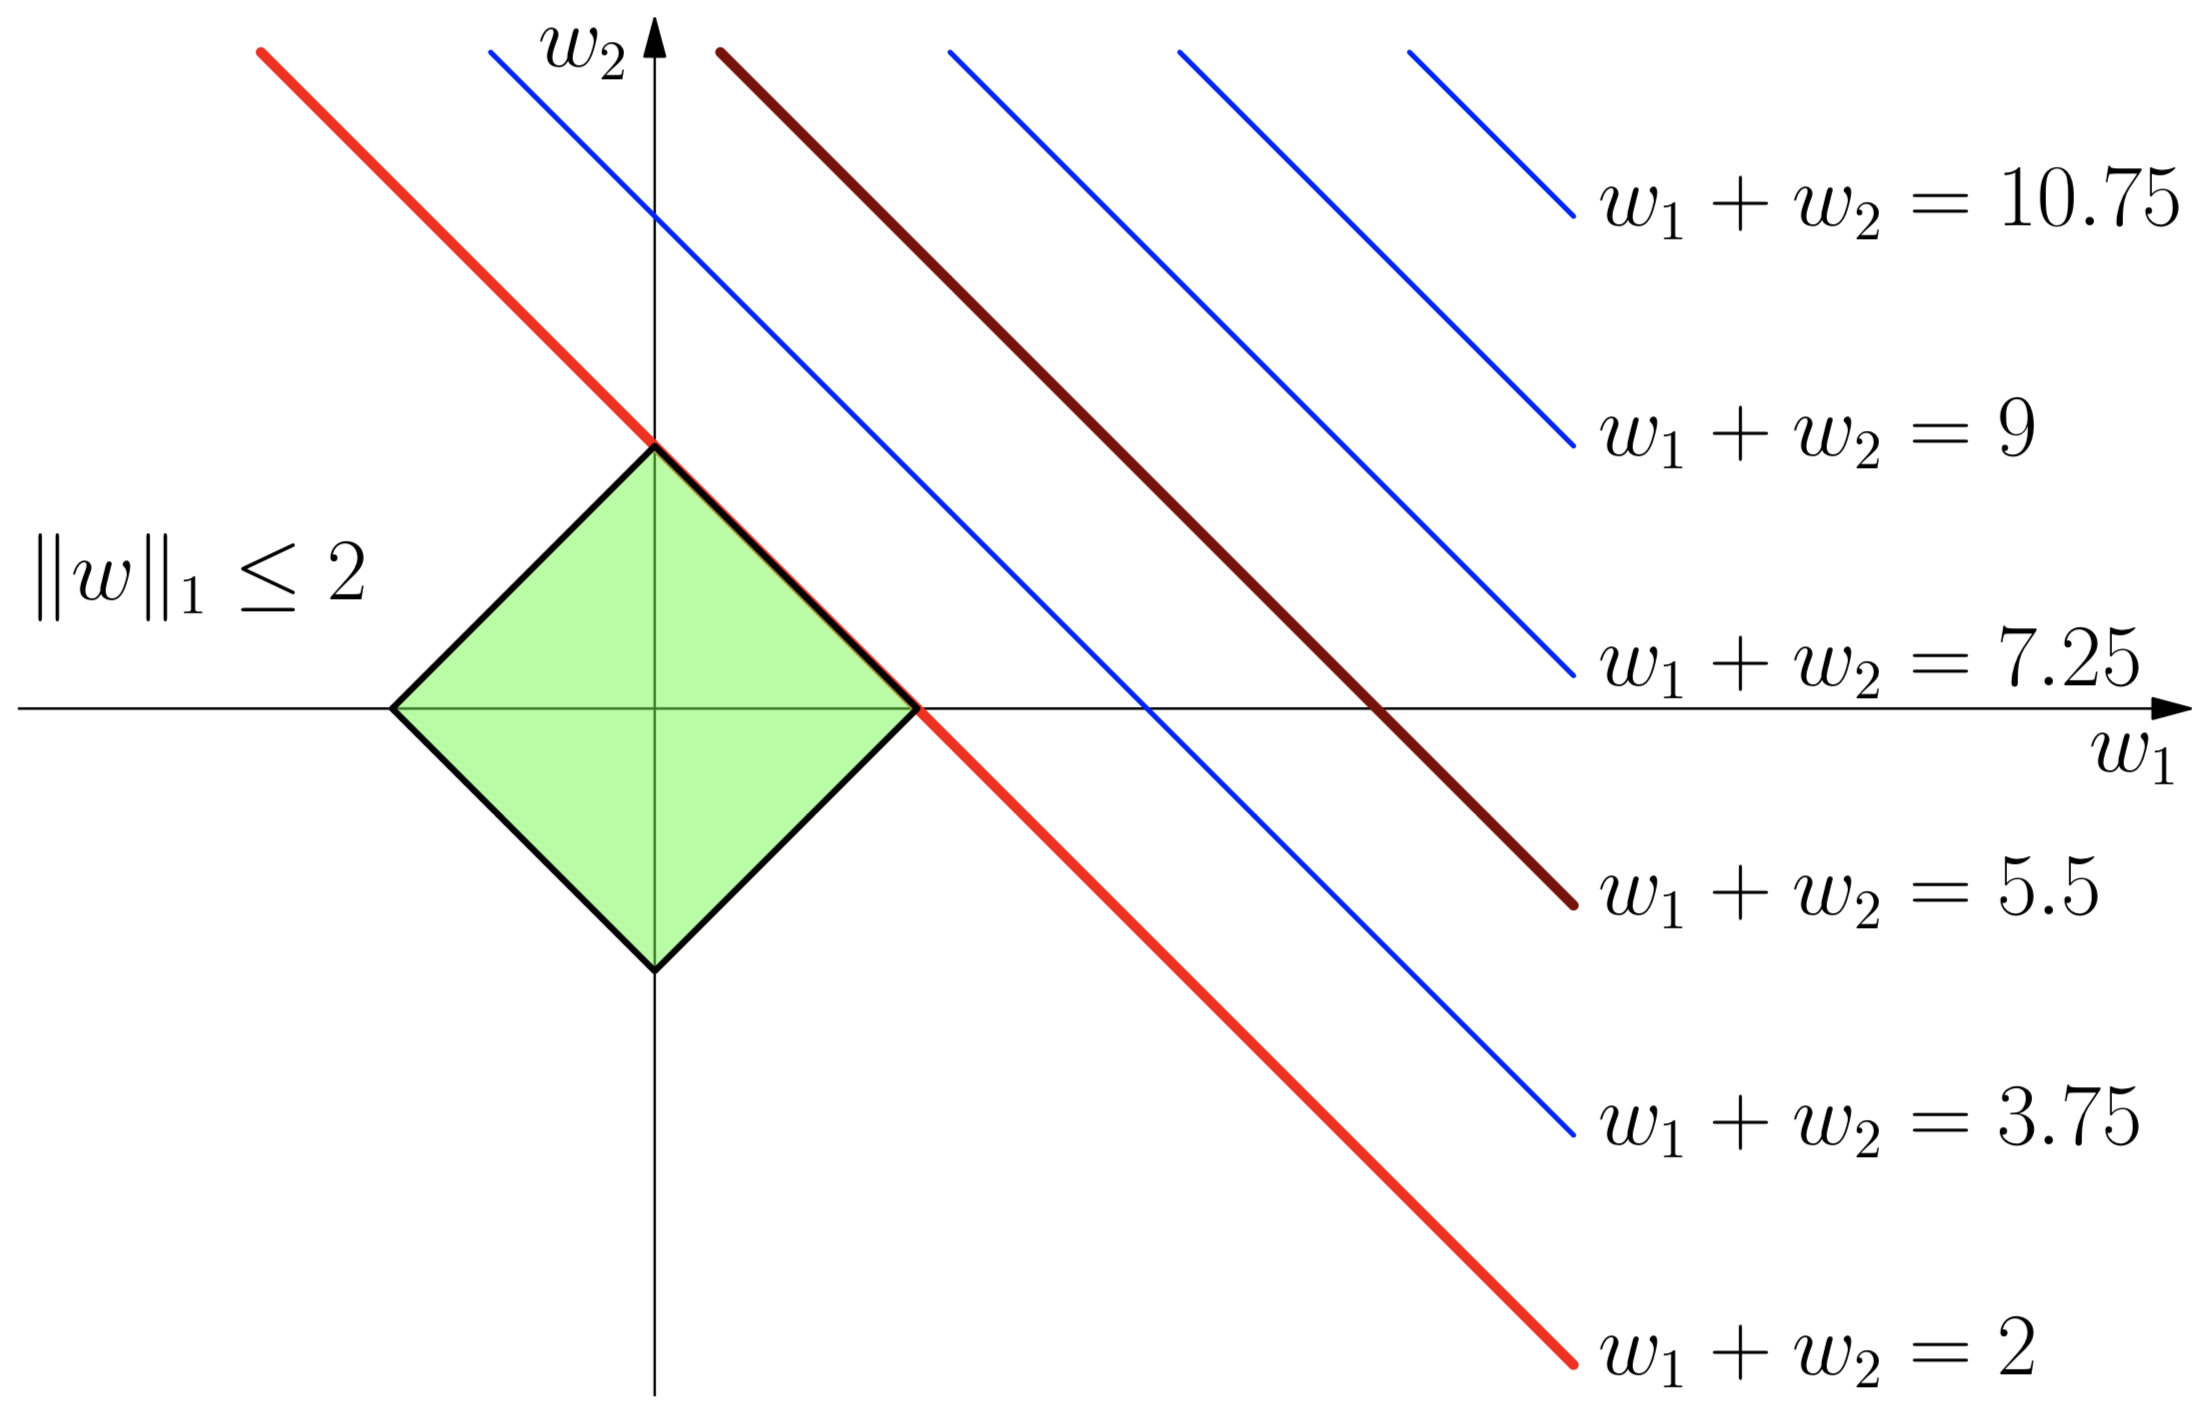
\includegraphics[height=0.4\textheight]{figures/L1Eq}
\par\end{center}
\begin{itemize}
\item Suppose the line $w_{1}+w_{2}=5.5$ corresponds to the empirical risk
minimizers.
\item Intersection of $w_{1}+w_{2}=2$ and the norm ball $\|w\|_{1}\le2$
is lasso solution.
\item Note that the solution set is $\left\{ \left(w_{1},w_{2}\right):w_{1}+w_{2}=2,w_{1},w_{2}\ge0\right\} $.
\end{itemize}
\end{frame}

\begin{frame}{Linearly Related Features}
\begin{itemize}
\item Linear prediction functions: $f(x)=w_{1}x_{2}+w_{2}x_{2}$
\item Same setup, now suppose $x_{2}=2x_{1}$.
\item Then all functions with $w_{1}+2w_{2}=k$ have the same empirical risk. 
    \note[item]{So $f(x)=w_{1}x_{1}+w_{2}x_{2}=w_{1}x_{1}+2w_{2}x_{1}=\left(w_{1}+2w_{2}\right)x_{1}$.
So all functions with $w_{1}+2w_{2}=k$ are the same.}
\item What function will we select if we do ERM with $\ell_{1}$ or $\ell_{2}$ constraint?
\end{itemize}
\end{frame}

\begin{frame}{Linearly Related Features, $\ell_{2}$ Constraint}
\begin{center}
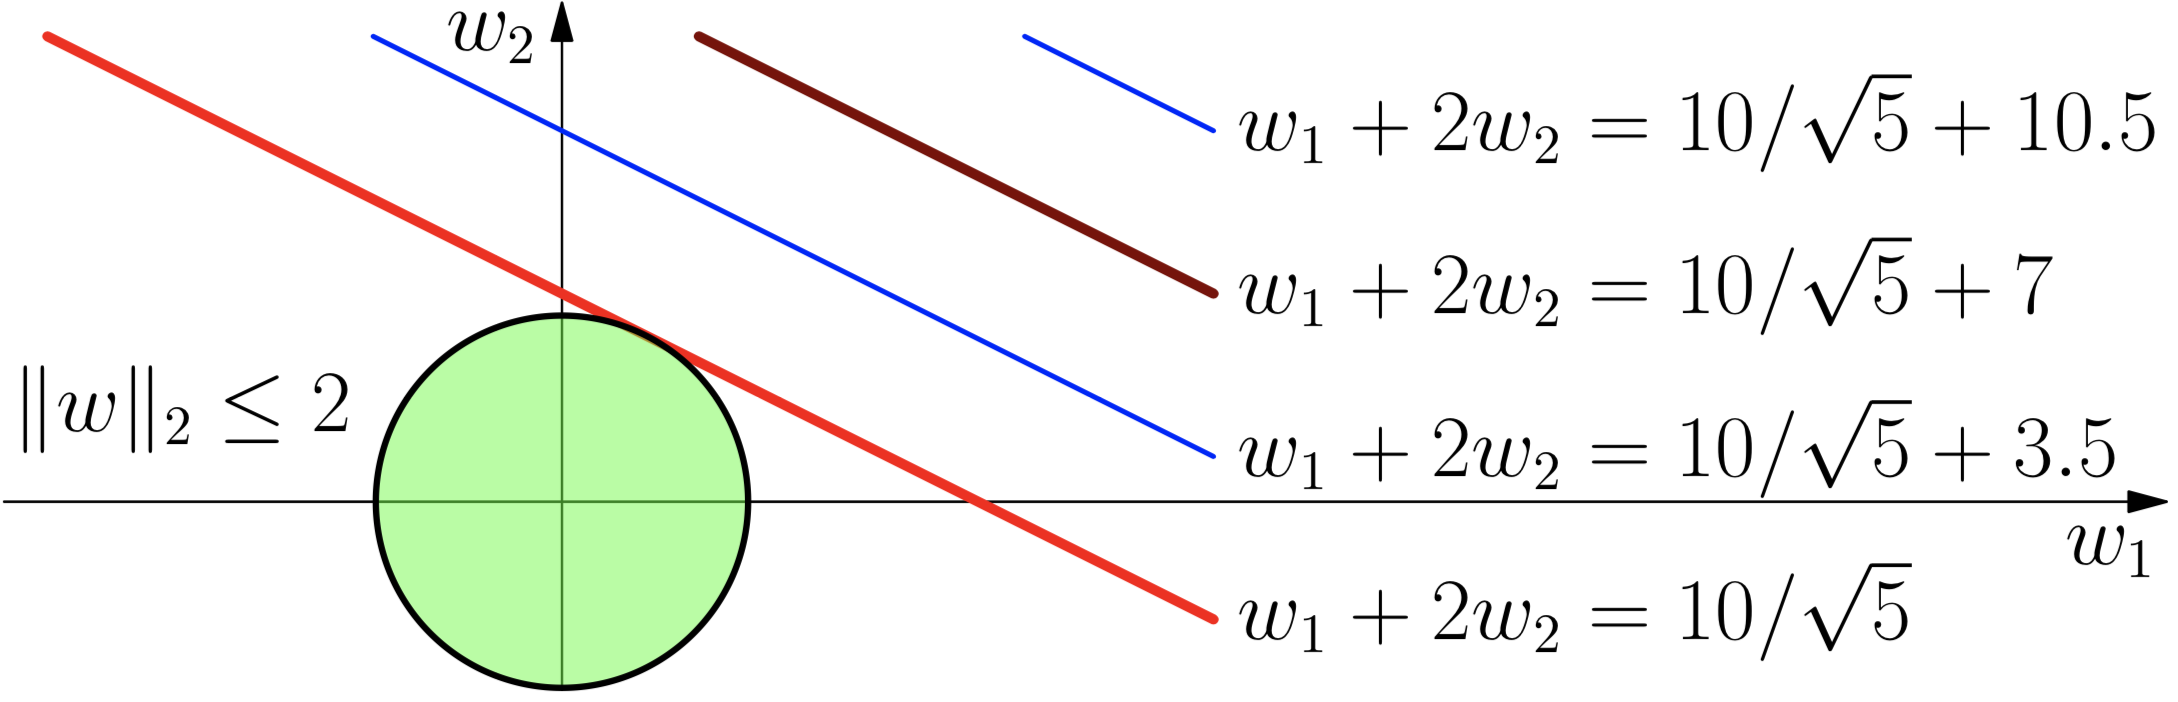
\includegraphics[height=0.4\textheight]{figures/L2Doub}
\par\end{center}
\begin{itemize}
\item $w_{1}+2w_{2}=10/\sqrt{5}+7$ corresponds to the empirical risk minimizers.
\item Intersection of $w_{1}+2w_{2}=10\sqrt{5}$ and the norm ball $\|w\|_{2}\le2$
is ridge solution.
\item At solution, $w_{2}=2w_{1}$.
\end{itemize}
\end{frame}
%
\begin{frame}{Linearly Related Features, $\ell_{1}$ Constraint}
\begin{center}
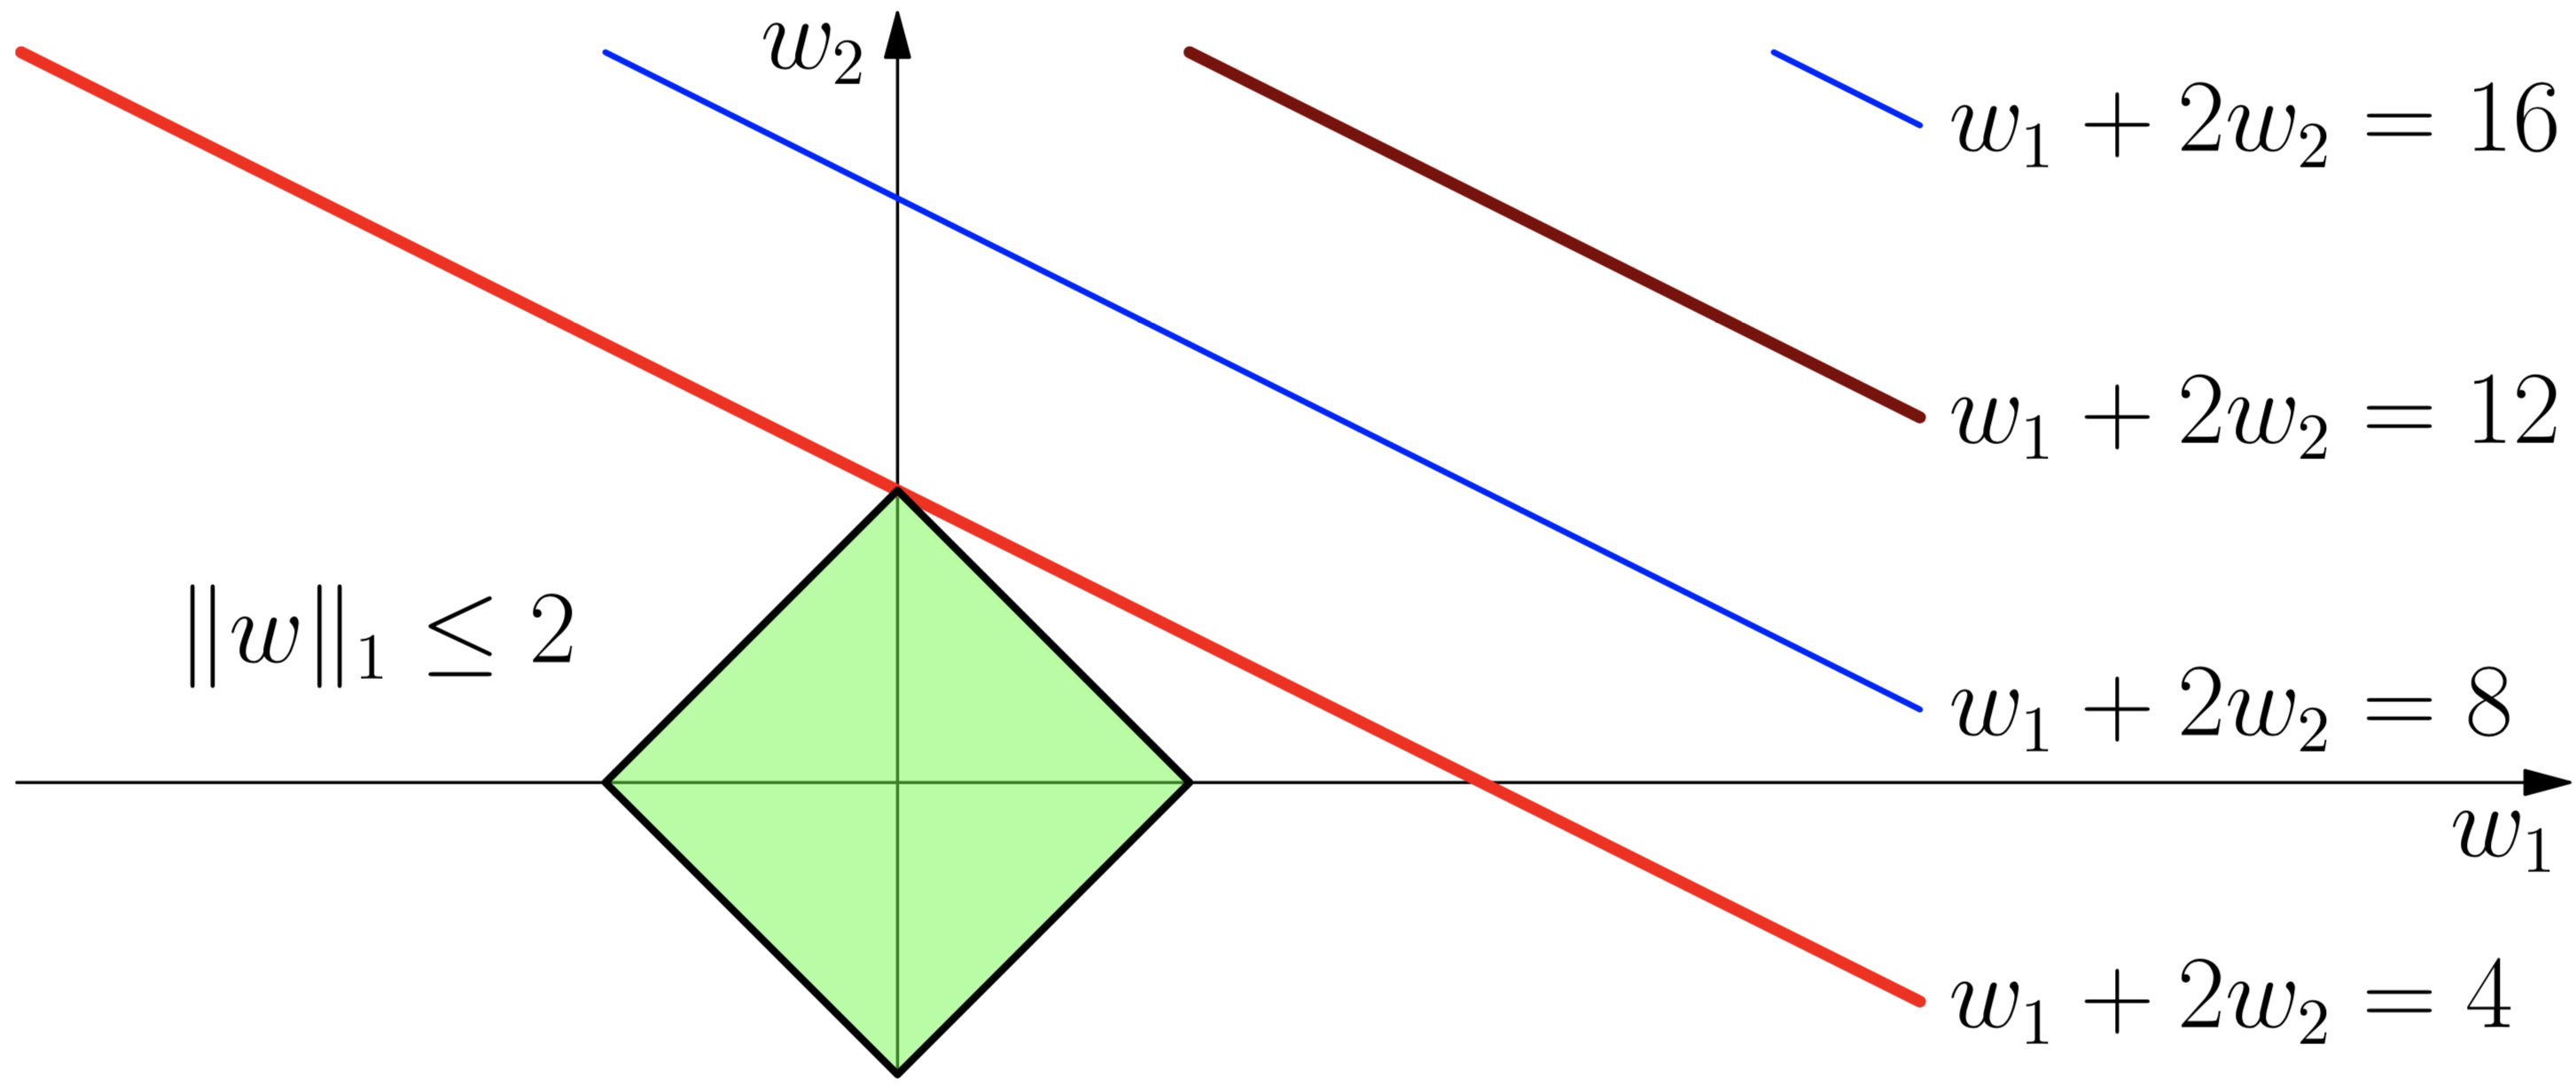
\includegraphics[height=0.4\textheight]{figures/L1Doub}
\par\end{center}
\begin{itemize}
\item Intersection of $w_{1}+2w_{2}=4$ and the norm ball $\|w\|_{1}\le2$
is lasso solution.
\item Solution is now a corner of the $\ell_{1}$ ball, corresonding to
a sparse solution.
\end{itemize}
\end{frame}

\begin{frame}{Linearly Dependent Features: Take Away}
\begin{itemize}
\item For identical features
\begin{itemize}
\item $\ell_{1}$ regularization spreads weight arbitrarily (all weights
same sign)
\item $\ell_{2}$ regularization spreads weight evenly 
\end{itemize}
\item Linearly related features
\begin{itemize}
    \item $\ell_{1}$ regularization chooses variable with \hl{larger scale}, 0 weight
to others
\item $\ell_{2}$ prefers variables with larger scale, spreads
    weight \hl{proportional to scale}
\end{itemize}

\item In practice, \textbf{feature standardization} is important.

\item How to standardize the test set?
        \note[item]{Use the training set statistics.}
\end{itemize}
\end{frame}

\begin{frame}{Correlated Features on Same Scale}
\begin{itemize}
\item Suppose $x_{1}$ and $x_{2}$ are highly correlated and the same scale.
\item This is quite typical in real data, after normalizing data. 
\end{itemize}

What do the level sets look like?\\
    \begin{itemize}
\item Nothing degenerate here, so level sets are ellipsoids. 
\item But, the higher the correlation, the closer to degenerate we get.
\item That is, ellipsoids keep stretching out, getting closer to two parallel
lines.
\end{itemize}
\end{frame}

\begin{frame}{Correlated Features, $\ell_{1}$ Regularization}
\begin{center}
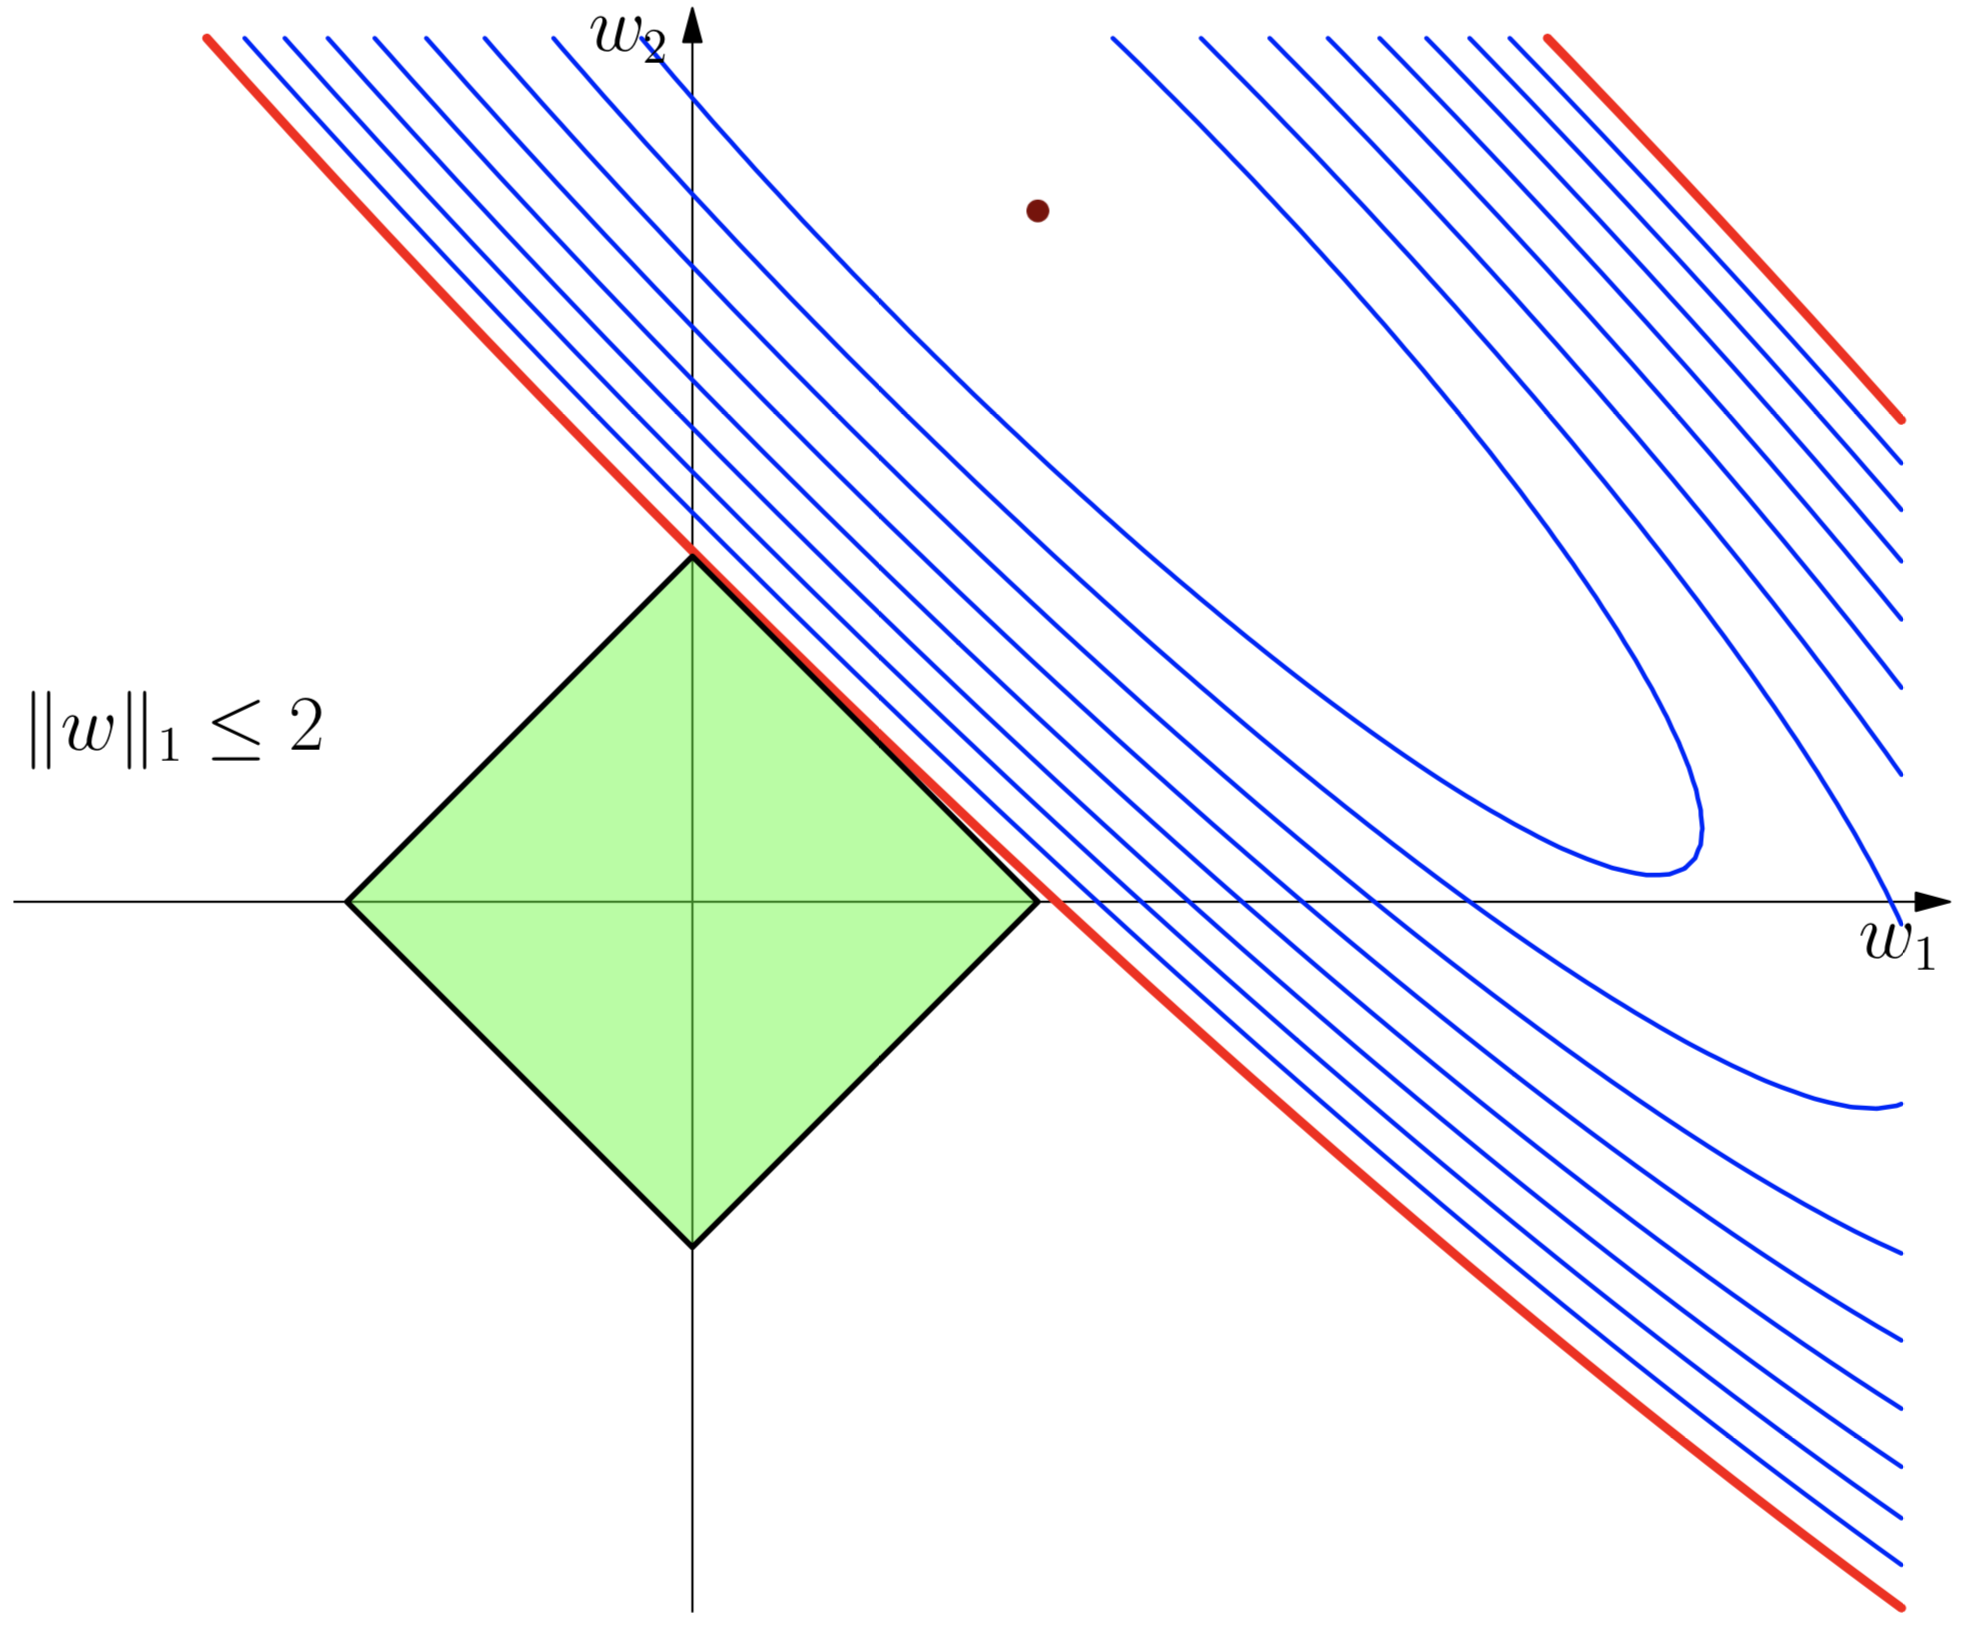
\includegraphics[height=0.4\textheight]{figures/L1Corr}\hspace{0.2\textwidth}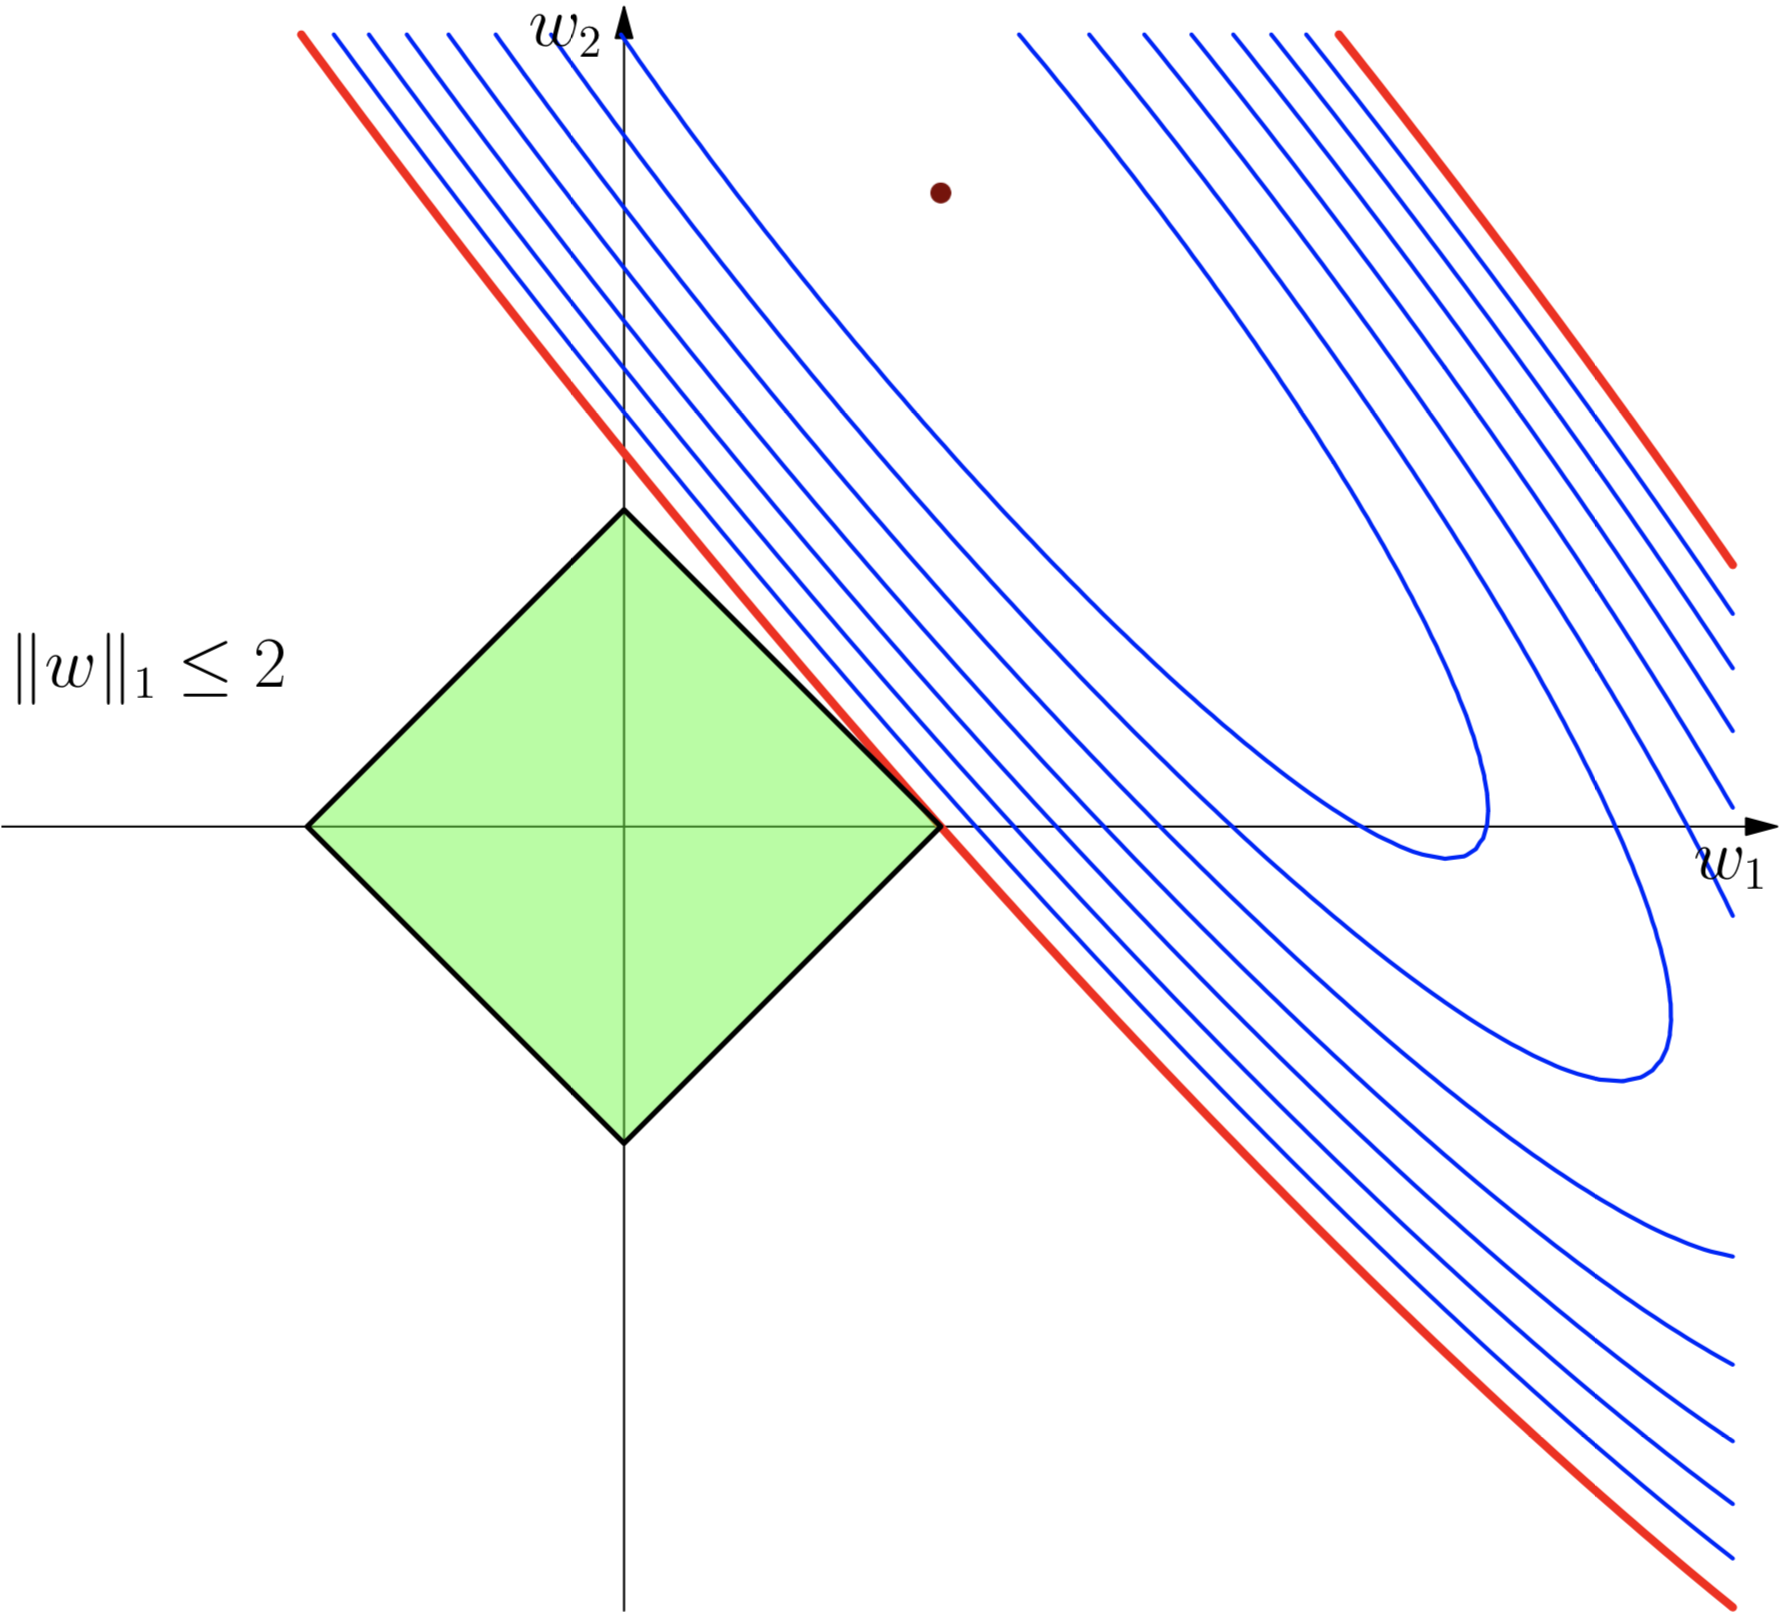
\includegraphics[height=0.4\textheight]{figures/L1Corr2}
\par\end{center}
\begin{itemize}
\item Intersection could be anywhere on the top right edge. 
\item Minor perturbations (in data) can drastically change intersection
point \textendash{} very unstable solution.
\item Makes division of weight among highly correlated features (of same
scale) seem arbitrary.
\begin{itemize}
\item If $x_{1}\approx2x_{2}$, ellipse changes orientation and we hit a
corner. (Which one?)
\end{itemize}
\end{itemize}
\end{frame}

\begin{frame}{Elastic Net}
The \textbf{elastic net} combines lasso and ridge penalties:
\[
\hat{w}=\argmin_{w\in\reals^{d}}\frac{1}{n}\sum_{i=1}^{n}\left\{ w^{T}x_{i}-y_{i}\right\} ^{2}+\lambda_{1}\|w\|_{1}+\lambda_{2}\|w\|_{2}^{2}
\]

What are the coefficients for correlated variables?

\note[item]{We expect correlated random variables to have similar coefficients.}
\end{frame}

\begin{frame}{Highly Correlated Features, Elastic Net Constraint}
\begin{center}
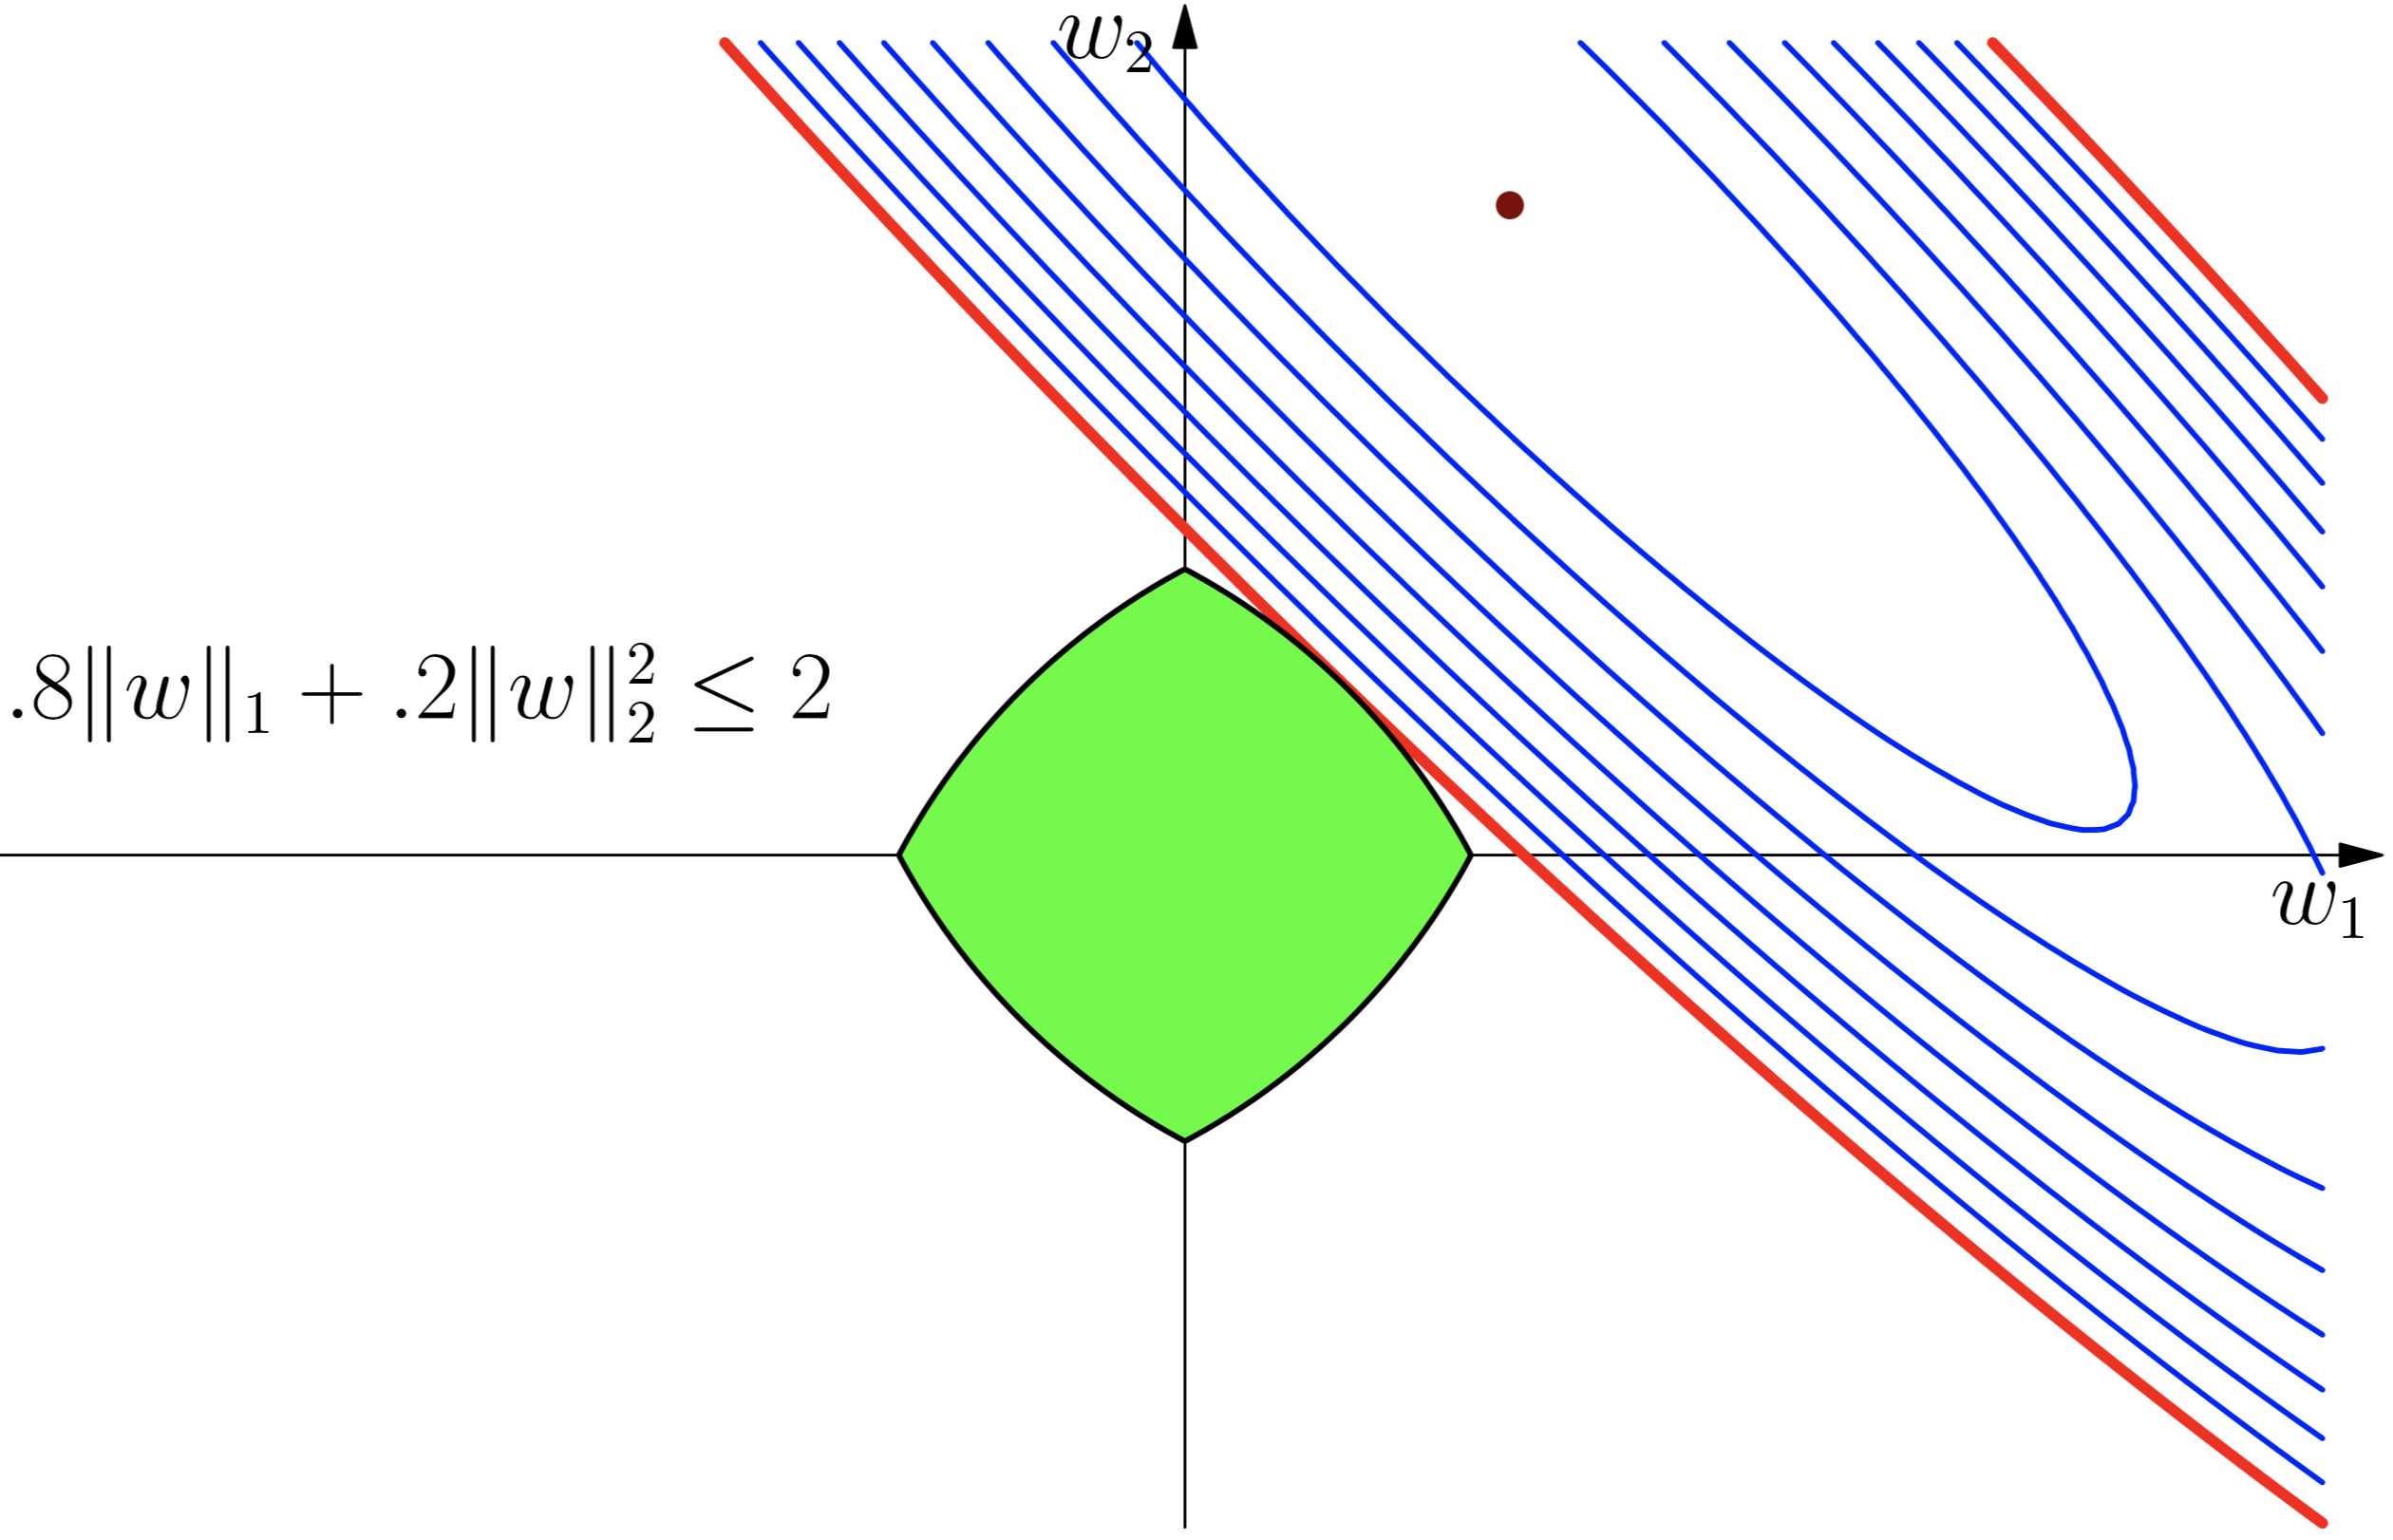
\includegraphics[height=0.5\textheight]{figures/EnetCorr}
\par\end{center}
\begin{itemize}
\item Elastic net solution is closer to $w_{2}=w_{1}$ line, despite high
correlation.
\item Elastic net selects variables like Lasso
\item And shrinks coefficients of correlated varialbes like Ridge
\end{itemize}
\end{frame}

\begin{frame}
    {Elastic Net vs $\ell_q$ Constraints}
    What if we use $\ell_q$ penalty where $q\in(1,2)$?
    \begin{figure}
        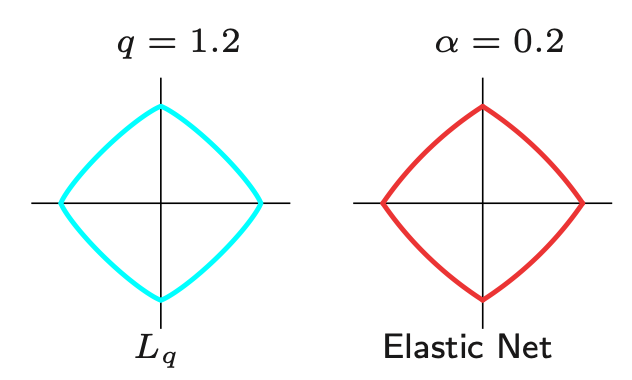
\includegraphics[height=0.5\textheight]{figures/elastic-lq}
    \end{figure}
    \note[item]{Although they look very similar, $\ell_q$ does not have sharp/non-differentiable corners thus cannot push weights to exactly zero.}
\end{frame}

\section{Sparsity}

\begin{frame}
    {Why doesn't $\ell_2$ give sparsity}
    Consider $\ell_2$ regularized least squares:
    \begin{align}
        L(w) = \frac{1}{2}\|Xw-y\|^2 + \frac{1}{2}\|w\|^2 .
    \end{align}

    Let $w^*$ be the optimal solution. What's the condition for $w_j^*=0$?
    \vspace{10em}
    \note[item]{We need
        \begin{align}
            \frac{\partial}{\partial w_j} L(w)\bigg|_{w_j=0} &= x_{\cdot j}^T(Xw - y) = 0
        \end{align}
        when $w_{-j}$ takes the optimal value.
        This requires the $j$-th features, $x_{\cdot j}$,
        to be orthogonal to the residual without using feature $j$,
        $X_{-j}w^*_{-j} - y$.
    }
    \note[item]{Note that the condition does not depend on $\lambda$.}
\end{frame}

\begin{frame}
    {Why does $\ell_1$ give sparsity}
    Consider $\ell_1$ regularized least squares:
    \begin{align}
        L(w) = \frac{1}{2}\|Xw-y\|^2 + \|w\|_1 .
    \end{align}
    Let $w^*$ be the optimal solution. What's the condition for $w_j^*=0$?
    \vspace{10em}
    \note[item]{We need
        \begin{align}
            \frac{\partial}{\partial w_j} L(w)\bigg|_{w_j=0} &= x_{\cdot j}^T(Xw - y) + \lambda [-1, 1]= 0
        \end{align}
        because subderivative $\partial |w_j|$ at $w_j=0$ is $[-1, 1]$.
        This only requires the $j-th$ features to be close to orthogonal to the residual, specifically the inner product is within $[-\lambda, \lambda]$.
        }
        \note[item]{Thus increasing $\lambda$ sets more weights to zero.} 
\end{frame}

\begin{frame}
    {Do we always want sparsity or simpler models?}
    \pause
    \begin{itemize}
        \item Subjective desire for parsimony: Occam's razor
        \item Avoid overfit: approximatin/estimation error trade-off
        \item No free lunch theorem
    \end{itemize}
    \vspace{9em}
\end{frame}


\end{document}
